\documentclass{standalone}
\usepackage{tikz}
\usetikzlibrary{arrows.meta, positioning, shapes.geometric, calc}
\usepackage{amsmath}

\begin{document}
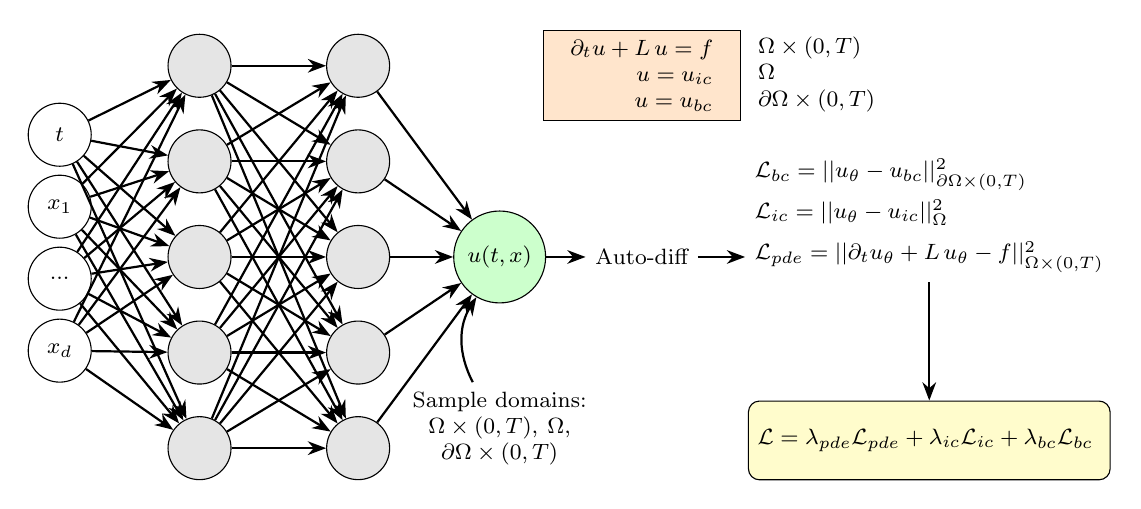
\begin{tikzpicture}[
  nn/.style={circle, draw, minimum width=0.5cm, minimum height=0.8cm, align=center},
  input/.style={nn, fill=white!20},
  hidden/.style={nn, fill=gray!20},
  output/.style={nn, fill=green!20},
  loss/.style={rectangle, draw, rounded corners, minimum width=2cm, minimum height=1cm, fill=yellow!20},
  every node/.style={font=\footnotesize},
  arrow/.style={-Stealth, thick}
]

% Inputs
\node[input] (input1) {$t$};
\node[input, below=0.1cm of input1] (input2) {$x_1$};
\node[input, below=0.1cm of input2] (input3) {...};
\node[input, below=0.1cm of input3] (input4) {$x_d$};

% Hidden layers
\node[hidden, above right=0.3cm and 1.2cm of input1] (h1) {};
\node[hidden, below=0.4cm of h1] (h2) {};
\node[hidden, below=0.4cm of h2] (h3) {};
\node[hidden, below=0.4cm of h3] (h4) {};
\node[hidden, below=0.4cm of h4] (h5) {};

% Hidden layers
\node[hidden, right=1.2cm of h1] (g1) {};
\node[hidden, below=0.4cm of g1] (g2) {};
\node[hidden, below=0.4cm of g2] (g3) {};
\node[hidden, below=0.4cm of g3] (g4) {};
\node[hidden, below=0.4cm of g4] (g5) {};

% Output
\node[output, right=0.8cm of g3] (output) {$u(t,x)$};

% Arrows for NN
\draw[arrow] (input1) -- (h1);
\draw[arrow] (input1) -- (h2);
\draw[arrow] (input1) -- (h3);
\draw[arrow] (input1) -- (h4);
\draw[arrow] (input1) -- (h5);
\draw[arrow] (input2) -- (h1);
\draw[arrow] (input2) -- (h2);
\draw[arrow] (input2) -- (h3);
\draw[arrow] (input2) -- (h4);
\draw[arrow] (input2) -- (h5);
\draw[arrow] (input3) -- (h1);
\draw[arrow] (input3) -- (h2);
\draw[arrow] (input3) -- (h3);
\draw[arrow] (input3) -- (h4);
\draw[arrow] (input3) -- (h5);
\draw[arrow] (input4) -- (h1);
\draw[arrow] (input4) -- (h2);
\draw[arrow] (input4) -- (h3);
\draw[arrow] (input4) -- (h4);
\draw[arrow] (input4) -- (h5);

\draw[arrow] (h1) -- (g1);
\draw[arrow] (h1) -- (g2);
\draw[arrow] (h1) -- (g3);
\draw[arrow] (h1) -- (g4);
\draw[arrow] (h1) -- (g5);
\draw[arrow] (h2) -- (g1);
\draw[arrow] (h2) -- (g2);
\draw[arrow] (h2) -- (g3);
\draw[arrow] (h2) -- (g4);
\draw[arrow] (h2) -- (g5);
\draw[arrow] (h3) -- (g1);
\draw[arrow] (h3) -- (g2);
\draw[arrow] (h3) -- (g3);
\draw[arrow] (h3) -- (g4);
\draw[arrow] (h3) -- (g5);
\draw[arrow] (h4) -- (g1);
\draw[arrow] (h4) -- (g2);
\draw[arrow] (h4) -- (g3);
\draw[arrow] (h4) -- (g4);
\draw[arrow] (h4) -- (g5);
\draw[arrow] (h5) -- (g1);
\draw[arrow] (h5) -- (g2);
\draw[arrow] (h5) -- (g3);
\draw[arrow] (h5) -- (g4);
\draw[arrow] (h5) -- (g5);

\draw[arrow] (g1) -- (output);
\draw[arrow] (g2) -- (output);
\draw[arrow] (g3) -- (output);
\draw[arrow] (g4) -- (output);
\draw[arrow] (g5) -- (output);

% Collocation points
%\node[below=1cm of h2] (colloc) {Collocation\\points $\Omega$};
%\draw[arrow] (colloc) to[bend right] (h1);

% Data points
\node[align=center, below=1cm of output] (data) {
  Sample domains:\\[0.0cm]
  $\Omega\times(0,T),\: \Omega,$\\[0.0cm]
  $\partial\Omega\times(0,T)$%\\[0.0cm]
  %$\Omega$
};
\draw[arrow] (data) to[bend left] (output);

% Auto-diff & residual
\node[right=0.5cm of output] (ad) {Auto-diff};
\node[right=0.6cm of ad] (r_pde) {$\mathcal{L}_{pde} = ||\partial_t u_\theta + L\,u_\theta - f||^2_{\Omega\times(0,T)}$};
\node[above right=0.05cm and 0.6cm of ad] (r_ic) {$\mathcal{L}_{ic} = ||u_\theta - u_{ic}||^2_{\Omega}$};
\node[above right=0.5cm and 0.6cm of ad] (r_bc) {$\mathcal{L}_{bc} = ||u_\theta - u_{bc}||^2_{\partial\Omega\times(0,T)}$};
\draw[arrow] (output) -- (ad);
\draw[arrow] (ad) -- (r_pde);
%\draw[arrow] (output) to[bend left] (r_ic);
%\draw[arrow] (output) to[bend left] (r_bc);

% Loss
\node[loss, align=center, below=1.5cm of r_pde] (lossbox) {
$\mathcal{L} = \lambda_{pde}\mathcal{L}_{pde} + \lambda_{ic}\mathcal{L}_{ic} + \lambda_{bc}\mathcal{L}_{bc}$
%$L_u = \|u - z\|_\Gamma$\\[0.2cm]
%$L_f = \|f\|_\Omega$
};
%\draw[arrow] ($(output.south east)!0.5!(r_pde.south west)$) -- (lossbox.north west);
\draw[arrow] (r_pde) -- (lossbox.north);
%\draw[arrow] (data) -- (lossbox.west);

% PDE example
\node[draw, rectangle, align=right, above=1.5cm of ad, fill=orange!20, minimum width=2.5cm] (pde) {
$\partial_t u + L\,u = f$\\[0.0cm]
$u = u_{ic}$\\[0.0cm]
$u = u_{bc}$
};
\node[align=left, above right=1.5cm and 0.0cm of ad, minimum width=3cm] (pde_domains) {
$\Omega\times(0,T)$\\[0.0cm]
$\Omega$\\[0.0cm]
$\partial\Omega\times(0,T)$
};

\end{tikzpicture}
\end{document}
